\documentclass[tikz,border=5]{standalone}
\usepackage{tikz}
\usetikzlibrary{
                arrows.meta,
                bending,
                positioning
               }
\tikzset{
         > = Latex,
         arrows = {[bend]},
         signal/.style = coordinate,
         sum/.style = {
                       draw,
                       circle,
                       minimum size = 2mm
                      },
         block/.style = {
                         draw,
                         rectangle,
                         minimum height = 2em,
                         minimum width = 4em
                        },
         branch/.style = {
                          sum,
                          minimum size = 1mm,
                          fill = black
                         }
        }

\begin{document}

  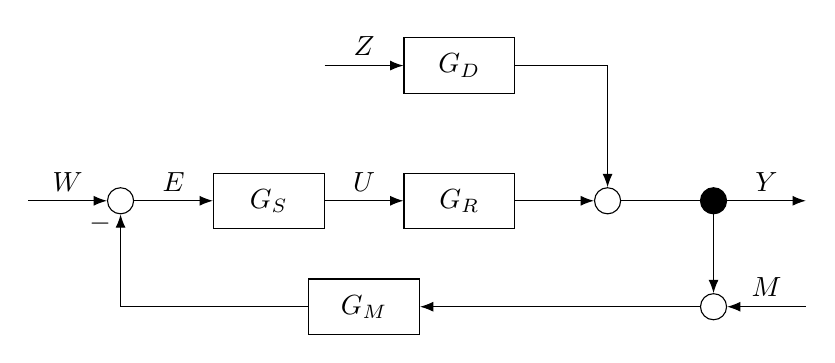
\begin{tikzpicture}[auto]

    %placing the nodes
    \node[signal] (input) {};
    \node[sum, right = of input] (left sum) {};
    \node[block, right = of left sum] (system) {$G_S$};
    \node[block, right = of system] (controller) {$G_R$};
    %connecting the controller and system to get the coordinates of u, its needed for the placement of the measurement block
    \draw
      [->] (system) -- node[name = u] {$U$} (controller);
    \node[block, above = of controller] (dynamic of disturbances) {$G_D$};
    \node[signal, left = of dynamic of disturbances] (disturbances) {};
    \node[sum, right = of controller] (right sum) {};
    \node[branch, right = of right sum] (branch) {};
    \node[signal, right = of branch] (output) {};
    \node[sum, below = of branch] (lower sum) {};
    \node[signal, right = of lower sum] (measurement noise) {};
    \node[block] (measurement) at (u |- lower sum) {$G_M$};
    %connecting the nodes
    \draw
      [->] (input) -- node {$W$} (left sum);
    \draw
      [->] (left sum) -- node {$E$} (system);
    \draw
      [->] (controller) -- (right sum);
    \draw
      [->] (disturbances) -- node {$Z$} (dynamic of disturbances);
    \draw
      [->] (dynamic of disturbances) -| (right sum);
    \draw
      (right sum) -- (branch);
    \draw
      [->] (branch) -- node {$Y$} (output);
    \draw
      [->] (branch) -- (lower sum);
    \draw
      [->] (measurement noise) -- node[above] {$M$} (lower sum);
    \draw
      [->] (lower sum) -- (measurement);
    \draw
      [->] (measurement) -| node[pos = .95] {$-$} (left sum);

  \end{tikzpicture}



\end{document}